\documentclass{article}

\usepackage{svg}
\usepackage[strict]{changepage}
\usepackage[none]{hyphenat}
\usepackage[style=authoryear,backend=biber]{biblatex}
\usepackage{graphicx}
\usepackage{subcaption}
\usepackage{booktabs}
\usepackage{listings}
\usepackage{float}
\usepackage{adjustbox}
\usepackage{wrapfig}

\newcommand{\codelocation}{../../../../Haskell/networked-poker}

\addbibresource{sections/bibliography.bib}
\setcounter{tocdepth}{1}
\setcounter{secnumdepth}{1}

\begin{document}

\lstset{language=Haskell,
        frame=single,
        captionpos=b
}

% taken from https://www.overleaf.com/latex/examples/title-page-with-logo/hrskypjpkrpd
\begin{titlepage}

\newcommand{\HRule}{\rule{\linewidth}{0.5mm}} % Defines a new command for the horizontal lines, change thickness here

\center{} % Center everything on the page
 
%----------------------------------------------------------------------------------------
%   HEADING SECTIONS
%----------------------------------------------------------------------------------------

\textsc{\LARGE University of Hull}\\[1.5cm] % Name of your university/college
\textsc{\Large A Networked Poker Game and AI}\\[0.5cm] % Major heading such as course name
%\textsc{\large Project Overview}\\[0.5cm] % Minor heading such as course title

%----------------------------------------------------------------------------------------
%   TITLE SECTION
%----------------------------------------------------------------------------------------

\HRule\\[0.4cm]
{\huge \bfseries Interim Report}\\[0.4cm] % Title of your document
\HRule\\[1.5cm]
 
%----------------------------------------------------------------------------------------
%   AUTHOR SECTION
%----------------------------------------------------------------------------------------

\begin{minipage}{0.4\textwidth}
\begin{flushleft} \large
\emph{Author:}\\
Zachary \textsc{Palmer} % Your name
\end{flushleft}
\end{minipage}
\begin{minipage}{0.4\textwidth}
\begin{flushright} \large
\emph{Supervisor:} \\
Dr.\ C. \textsc{Kambhampati} % Supervisor's Name
\end{flushright}
\end{minipage}\\[2cm]

\textsc{\large Submitted for the BSc in Computer Science}\\[0.5cm]

% If you don't want a supervisor, uncomment the two lines below and remove the section above
%\Large \emph{Author:}\\
%John \textsc{Smith}\\[3cm] % Your name

%----------------------------------------------------------------------------------------
%   DATE SECTION
%----------------------------------------------------------------------------------------

{\large \today}\\[0.5cm] % Date, change the \today to a set date if you want to be precise

{\large Word Count: 4892}\\[2cm]

%----------------------------------------------------------------------------------------
%   LOGO SECTION
%----------------------------------------------------------------------------------------

%
\includegraphics{logo.png}\\[1cm] % Include a department/university logo - this will require the graphicx package
\includesvg{logo.svg}\\[1cm]
 
%----------------------------------------------------------------------------------------

\vfill % Fill the rest of the page with whitespace

\end{titlepage}


\tableofcontents
\newpage

\section{Introduction}
This report will set out to detail the developed software: A poker server,
client with GUI, and a simplistic AI\@. Test programs were also developed
to illustrate the performance of different card picking algorithms and sources
of randomness. The reasons behind design and architectural choices, along with 
evidence to support these, assisted by the extra programs will be detailed. 
Sections covered will be the current progression of the project according to
the previously created time plan, the gameplay, the GUI interface, and an in 
depth look at randomness and card generation.

\newpage

\section{Graphical User Interface Design}
Designing the graphical interface began with simple mockups. A simple
initial diagram is shown below.

\begin{figure}[h]
    \frame{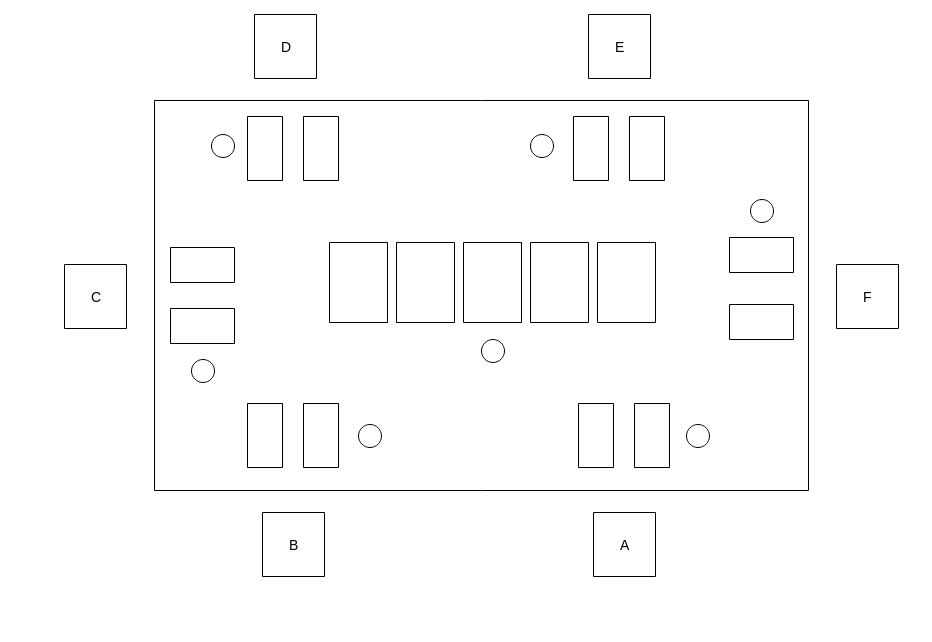
\includegraphics[width=\linewidth]{../images/initialgui.png}}
    \caption{Initial GUI mockup}%
    \label{fig:initialgui}
\end{figure}

This is a very standard design which cannot be varied much. All players have
two cards, a current bet, and a total amount of chips. As you may notice
in Figure~\ref{fig:initialgui} there is no label for the players total amount
of chips. This was instead decided to be stored as part of the name component,
as it makes for much less visual noise. The player labelled `A', is the
users player. He/she will always be seated here, and the other players will
be rotated around the board from their perspective. That is, every single
player A through F will appear to be in seat A from their own point of view.
The GUI is player centric. The relative positions, however will not be 
modified. Player A will always have player B to their left and Player F to 
their right, no matter where they visually appear to be. Of course, this has 
been implemented to not affect how the gameplay works, as the ordering of 
players is maintained, it is simply the visual representation of the players 
which is being manipulated.

The players need some way to interact with the game, and simple buttons which 
lie under the poker table were used for this. The raise button brought some 
complications, as the user has to enter a valid integer to increase the current
bet to. Some constraints are placed on this parameter.

\newpage

\begin{itemize}
\item The user must have enough chips to make the raise
\item The user must raise by at least the minimum raise
\item The raise must be an integer, not fractional
\end{itemize}

It was decided to use a separate window with a slider to handle the above
reasons. A slider has a minimum, and a maximum. This prevents the user from
both raising too little, and too much. And, by setting a slide interval, it
prevents the user selecting a non integer.

\begin{figure}[h]
    \centering
    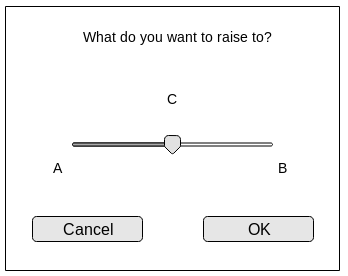
\includegraphics[width=0.5\linewidth]{../images/raisewindow.png}
    \caption{The Raise Window}%
    \label{fig:raisewindow}
\end{figure}

However, in the implementation of this, it was found that when displaying
the selected value, despite the steps being integer steps of one, 
fractional values could arise due to inherent errors in floating point 
mathematics. This was solved by simply taking the raw slider value, and 
casting it to an integer variable. This variable was then used for displaying 
the current users selection, and for the program to take as the chosen value 
once the `OK' button had been selected. Figure~\ref{fig:raisewindow} shows the 
raise window, where A is the minimum value, B is the maximum value, and C is 
the current value.

\begin{figure}
    \centering
    \begin{subfigure}[h]{0.4\textwidth}
        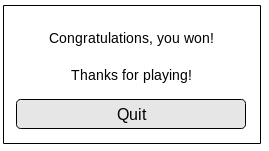
\includegraphics[width=\textwidth]{../images/winscreen.png}
        \caption{The Win Window}%
        \label{fig:winwindow}
    \end{subfigure}
    \begin{subfigure}[h]{0.4\textwidth}
        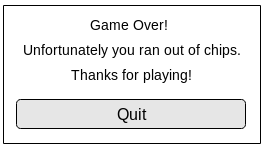
\includegraphics[width=\textwidth]{../images/lossscreen.png}
        \caption{The Loss Window}%
        \label{fig:losswindow}
    \end{subfigure}
    \caption{The Game Over Windows}\label{fig:gameoverwindows}
\end{figure}

Finally, there were elements needed for when a player either wins the game,
by the other players being eliminated for running out of chips, or when a
player loses, by being eliminated themselves. These took the form of simple
windows with configurable text, and a quit button. Both the win window
and the loss window use the same component, with only differing text. This
keeps the GUI consistent, and thus increases user acceptance.

Once the mockups had been completed the GUI was implemented in QtQML,
and hooked up to the Haskell code so it was fully usable and could be used
to test the poker game. Figure~\ref{fig:actualgui} shows the GUI in use,
with 6 players participating in a game. 

\begin{figure}[h]
    \centering
    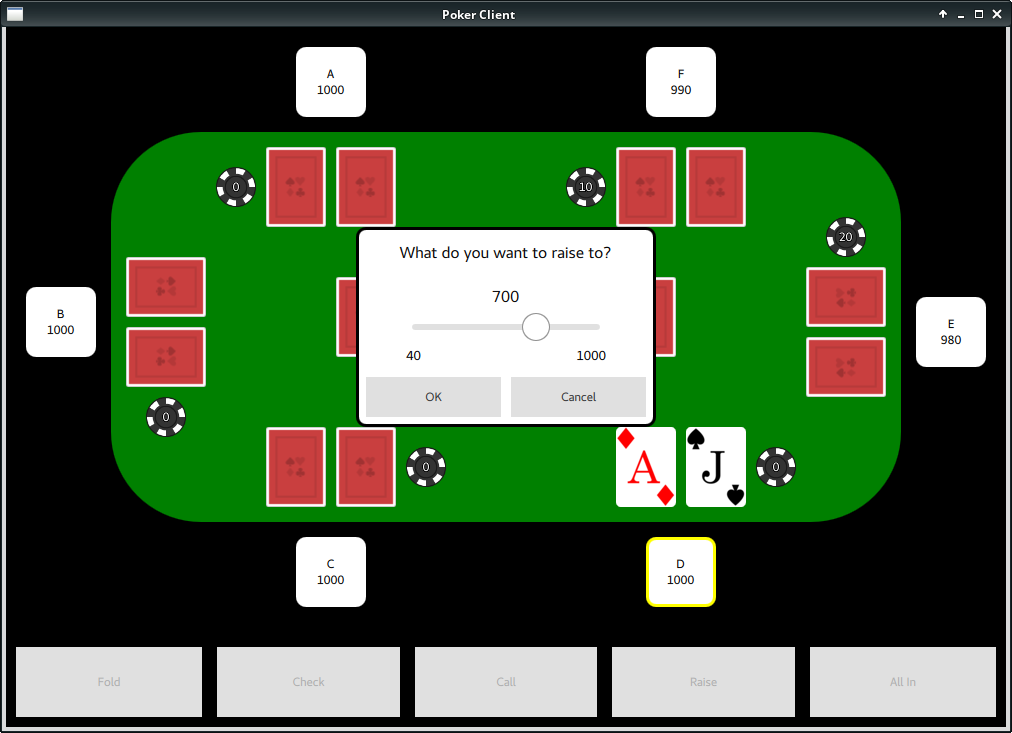
\includegraphics[width=\textwidth]{../images/actualgui.png}
    \caption{The initial implemented GUI}%
    \label{fig:actualgui}
\end{figure}

You can also see the implemented raise window in this image. Aside from the 
obvious card and poker chip assets, and colours, the implemented GUI is 
essentially the same as the mockup. One difference that was decided upon 
adding whilst testing, was a yellow border around the current player, so users 
would know how long it was until it was their turn. 

One feature of note is button fading. When buttons are unavailable, for
example if it's not the players turn, or a certain action would be invalid,
the buttons are greyed out, and unclickable. When actions become available,
they are clickable and fully coloured. This is an easy way to let players
know the valid actions whilst keeping the GUI consistent. Faded and non faded
buttons can be seen in figure~\ref{fig:guiwithconsole}.

Another modification considered making was adding a dealer chip. Whilst
online poker does not have an actual player who deals the cards, and indeed
in real life poker the dealer is often not an actual player, the concept of
a dealer is still used.

Each round, the dealer progresses, and the player to
the left of the dealer is the player who bets first. In the preflop, this
player has to play a forced blind, but once in the flop and beyond, this player
gets to bet first, which is of some strategic importance. 

For these reasons, a dealer chip would seem obvious, however it was decided
against, because it both clutters the GUI, and the dealer can still be
recognised by simply observing who plays the small blind, and retaining this
information, knowing the dealer progresses once to the left each full round.
In the above screenshot for example, the dealer can be identified to be A,
as the player to his left has played a small blind of 10 chips.

One modification that was added after the initial implementation was a text
console. This was used because some important information was difficult to 
display graphically, had to be interpreted very quickly, or was useful to be 
consulted at a later point in the game. The text console allowed messages such 
as bet history and hand values to be constantly visible to allow players to 
digest at their own pace.

\begin{figure}[h]
    \centering
    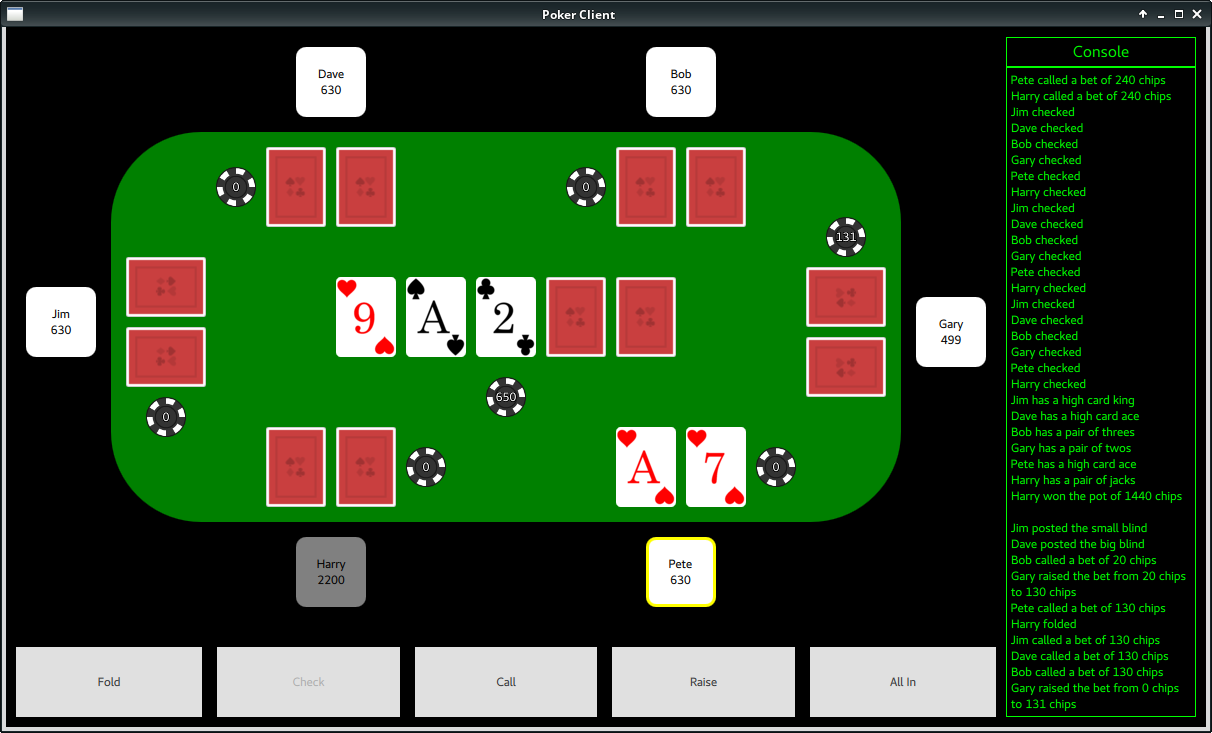
\includegraphics[width=\textwidth]{../images/guiwithconsole.png}
    \caption{The GUI with text console}%
    \label{fig:guiwithconsole}
\end{figure}

\newpage

\section{Gameplay}

\newpage

\section{Randomness and Shuffling}
In the game of poker, the house does not wager against players, unlike other 
popular casino games, such as blackjack or roulette, but instead the usual 
method for online poker companies and indeed poker tables in real life to make 
money is the rake. 

The implementation of the rake varies between casinos and online poker
software. Some common ones are in the below table.

\begin{center}
    \begin{tabular}{l l}
    \toprule
    Mechanism           & Description                                               \\
    \midrule
    Pot Rake            & Percentage taken from the pot, per hand or betting round  \\ \addlinespace
    Dead Drop           & Fee paid by the player with the dealer button each hand   \\ \addlinespace
    Timed Rake          & Set fee collected every set interval of time              \\ \addlinespace
    Fixed Fee           & Fixed fee per hand                                        \\ \addlinespace
    Tournament Fee      & Entry fee to participate in poker tournaments             \\ \addlinespace
    Subscription Fees   & Players are charged a subscription fee to play            \\
    \bottomrule
    \end{tabular}
\end{center}

Finally, some games are rake free, instead generating revenue by driving
traffic to more profitable businesses. The software developed that this paper
is discussing is also rake free, due to being only for academic purposes.

However, despite companies being able to generate revenue in these ways, the
implementation of random number generation in poker software is a topic of
some interest. Possible issues include rogue employees writing malicious
code to give them or people connected to them beneficial cards, faulty code
allowing the random number generation to be exploited, and other schemes, such
as giving newer players or failing players better cards, to encourage them to 
continue using the companies platform, and generating revenue through rakes.

For these reasons, random number generation has been analysed and multiple
different shuffling algorithms or card picking algorithms have been
developed and contrasted for possible weaknesses. Two obvious approaches to 
selecting cards are:

\begin{itemize}
    \item Storing an array of all the cards and indexing this array in some way to take a card
    \item Shuffling an array in some way and taking the top item
\end{itemize}

Multiple versions of both these algorithms have been implemented, using
different sources of randomness. In Haskell, the class keyword is analogous
to an interface in Object Orientated Languages, it defines functions that
an instance of the class must implement. Using the below class, multiple
implementations of card picking algorithms can be developed, and very simply
tested by calling the same functions, and only changing the instance used.

\vbox{%
\lstinputlisting[firstline=19, lastline=27, caption=Drawable]
                {\codelocation/server/src/lib/DrawCard.hs}
}

In the above code, the internal cards are encapsulated in a Deck, which
prevents users of the module modifying them, as the type constructor is not
exported. This means we can maintain state of the deck that users pass in
without having to resort to non Haskell-like code such as top level mutable
IORefs and unsafePerformIO\@.

The function initDeck returns an IO instance of Drawable. This function is 
used to initiate the deck, which involves a transform of some form upon the 
full deck. In the case of a Knuth shuffle, this would be shuffling the deck 
using the Knuth method \parencite{knuth1997}.

The function draw takes an instance of Drawable that was obtained from the
initDeck function or another invocation of draw, and draws a card in some way.
It then returns the card, and the new state of the instance. In the case of
a shuffle, this would generally just involve taking the first card of the
deck. Both these functions need to be in the IO Monad as generating random
numbers without a fixed seed involves IO\@.

Below are two implementations of the Drawable class, the first takes
random indexes from a deck and returns that card, the second uses the Knuth
shuffle to shuffle the deck then takes the top item from the deck.
\newline

\vbox{%
\lstinputlisting[firstline=29, lastline=41, caption=RandomIndex]
                {\codelocation/server/src/lib/DrawCard.hs}
}

\vbox{%
\lstinputlisting[firstline=43, lastline=64, caption=KnuthShuffle]
                {\codelocation/server/src/lib/DrawCard.hs}
}

\newpage

\section{Networking}

\newpage

\nocite{*}


\printbibliography[heading=bibintoc]

\end{document}
